\documentclass[13pt]{article}
\usepackage{amsmath}
\usepackage{amssymb}
\usepackage{amsthm}
\usepackage{color}
\usepackage{graphicx}
\title{A phylogenetic and population genetic model of amino acid substitution}
\author{}
\begin{document}
\maketitle
%%%%%%%%%%%%%%%%%%%%%%%%%%%%%%%%%%%%%%%%%%%%%%%%%%%%%%%%
\section{Abstract}
A new mechanistic model for the evolution of amino acid sequences is developed for studying the biological properties of proteins as well as phylogenetic estimation.  Two steps are bridged together to form a Markov process to describe substitutions between amino acids: mutation is based on general time reversible models for underlying nucleotides; fixation is obtained using classical population genetics theory. Selective restraints at amino acid level are characterized by the physiochemical distances between amino acids and the Grantham sensitivity coefficient exerted on the distances. Analysis of a yeast data set shows that the new model provides a better fit to data than the empirical models and reveals the variance of Grantham sensitivities and optimal amino acids at different sites in proteins.\\

\section{Introduction}
Importance of building accurate model for protein evolution. \\

Known models of amino acid replacement can be divided into two categories: empirical models and mechanistic models. Models in the first category include Dayhoff, JTT, WAG, LG, etc. Yang et al. (1998) implemented a few mechanistic models at the level of codons and explicitly modeled the biological processes involved, including different mutation rates between nucleotides, translation of the codon triplet into an amino acid, and the acceptance or rejection of the amino acid due to selective pressure on the protein. \\

Mechanistic models for the evolution of protein-encoding sequences are on three levels: mono-nucleotide level in DNA sequences, codon level in DNA coding sequences and amino acid level in protein sequences. Models on the DNA level use the most information and are more powerful to distinguish closely related sequences such as those caused by synonymous substitutions which are invisible at amino acid level. On the amino acid level, models can filter out some stochastic noise through the translation of DNA triplets to amino acids. Goldman and Yang (1994, MBE) constructed a codon-based model that uses the nucleotide-level information in DNA sequences and the amino-acid level information of synonymous and non synonymous nucleotide substitutions simultaneously. Their model incorporated transition / transversion bias, synonymous / nonsynonymous variation in a gene, and amino acid differences. The selective restraints at the amino acid level was accounted for by multiplying the substitution rate by a factor $\exp (d_{aa_i,aa_j}/V)$ where $d_{aa_i, aa_j}$ is the distance between amino acids $aa_i$ and $aa_j$ given by Grantham (1974) and $V$ is a parameter representing the variability of the gene or its tendency to undergo non synonymous substitution.\\

In Goldman and Yang's model, the Markov process is time reversible. In other words, the amino acids are equally as good in a protein and the substitution rates are  only proportional to the frequencies of the amino acids. However, from population genetics, the selective restraints should be a function of the fitness of proteins. Proteins with higher fitnesses get fixed with higher probability than those with low fitnesses. Gilchrist (2007) showed that the fitness of a protein is a function of factors including protein production cost, gene expression level, and functionality of protein. A protein might have a sequence of ``optimal" amino acids which give the protein best functionality, while other amino acids might also make the protein function but less well. Therefore, the functionality of a protein depends on what the optimal amino acids are and how far away the observed amino acids are from the optimal ones, as well as how sensitive the functionality is to the distance between amino acids. \\

In addition, the measure of difference between amino acids combines physiochemical properties that correlate best with protein residue substitution frequencies: composition, polarity and molecular volume. Grantham (1974) assigned weights to these three factors based on the average chemical distance given by the corresponding property alone. Take the composition for example, given the values for this property $c_i$'s, the weight $\alpha = (1/\bar{D}_c)^2 = 1.833$ where $\bar{D}_c = \sum[(c_i - c_j)^2]^{1/2}/190$. Similarly the weights for polarity and molecular volume are $0.1018$ and $0.000399$. Since the values for the volume property is much bigger than the other 2 properties its weight is much smaller. We call the weights Grantham weights. It is reasonable to believe that in some genes one property might play a more important role while in some genes it might be another property. For example ?  We present a new model that incorporates the above factors by including the Grantham weights $\alpha, \beta, \gamma$ and the sensitivity of functionality to distance from the optimal amino acid as parameters. We call the sensitivity coefficient ``Grantham sensitivity'' and denote is by $g$.\\

In this paper we characterize our amino acid-based model, which incorporates substitution rates of underlying coding nucleotides, the biological properties of amino acids, selection sensitivity of amino acid differences. We use the model for maximum likelihood (m.l.) estimation of phylogenies and apply the model to Rokas's yeast data sets with 8 species. The results are compared with those under previous amino-acid models. We also investigate the evolution process of protein with different parameters.\\
(and use simulations and information from empirical data to find cases where populations of intermediate size may evolve faster than populations of large size.)

%%%%%%%%%%%%%%%%%%%%%%%%%%%%%%%%%%%%%%%%%%%%%%%%%%%%%%%%
\section{Model}
Our model works for homologous protein-coding sequence without gaps or with gaps removed. We use a continuous time Markov process to model substitutions among the amino acids within a protein coding sequence. The states of the Markov process are the 20 natural amino acids (nonnatural amino acids can be easily added), so we use a $20 \times 20$ rate matrix $Q=(Q_{ij})$ where $Q_{ij}$ represents the instantaneous rate that amino acid $i$ will be substituted by amino acid $j$. The rate matrix $Q$ is obtained by multiplying the mutation rate matrix $M$ and fixation probability matrix $F$. As usual the row sum of $(Q_{ij})$ equals $0$ and $P(t) = \exp (tQ)$, where $P_{ij}(t)$ is the probability that amino acid $j$ replaces $i$ after time $t$.\\

Based on the $4 \times 4$ general time reversible (GTR) mutation rate matrix $M_{nu}$ for nucleotides the mutation rates $\mu_{ij}$ among 20 amino acids are calculated. We assume that mutations occur independently between nucleotides at the same codon position. Therefore, more than one nucleotide substitutions are not allowed to occur instantaneously as mutations involving more than one position during time $\Delta t$ will have probabilities on the order of $\Delta t^2$ and are, therefore, ignored. The calculation follows two steps. First, a $61 \times 61$ (stop codons not included) codon mutation rate matrix $M_{\text{codon}}$ is obtained; Second, using the genetic code table, we generate the $20 \times 20$ mutation rate matrix $M$ for all amino acids. The mutation process is time reversible, i.e. $\pi_i M_{ij} = \pi_j M_{ji}$ is satisfied for all $1 \le i, j \le 20$.\\

In addition to the effects of mutation bias our model also includes the effects of natural selection on the amino acid sequence of a gene. We begin by assuming that there is an optimal amino acid for each position in a protein and non-optimal amino acids each position are subjected to natural selection. The strength of selection depends on the scaled physiochemical distance (Grantham, Science 1974) between the observed and optimal amino acids, the sensitivity of the protein's function to the physicochemical distance and the protein production rate of the gene. \\

Suppose a protein of length $n$ has the optimal amino acid sequence $\hat{\mathbf{a}} = (\hat{a}_1, \hat{a}_2, \cdots \hat{a}_n)$, the observed sequence of amino acids is $\mathbf{a} = (a_1, a_2, \cdots, a_n)$, the Grantham sensitivity coefficient is $g_k$ and let $\mathbf{g}=(g_1,g_2,\cdots,g_n)$. The overall physiochemical difference (distance) between amino acids $i$ and $j$ consist of 3 components: $d_{ij} = [\alpha (c_i-c_j)^2 + \beta (p_i - p_j)^2 + \gamma (v_i - v_j)^2]$, where $c, p$ and $v$ represent physicochemical properties composition, polarity and molecular volume of the amino acid's side chain, and $\alpha, \beta, \gamma$ are the corresponding weights for the components. The values for physicochemical properties in the amino acid difference formula is given by Grantham (1974), each of them is weighted by dividing by the mean distance found with that property alone. In our model, the weights $\alpha, \beta, \gamma$ are treated as estimable parameters rather than being fixed. \\

The distance vector $\mathbf{d} = (d_1, d_2, \cdots, d_n)$ represents the distance per amino acid basis from the optimal and the Grantham sensitivity is $\mathbf{g}$. The functionality of a protein $\mathbf{a}$ with $n$ amino acids is defined as

\begin{equation}
F(\mathbf{a}| \hat{\mathbf{a}},\mathbf{g})  =  \frac{n}{\displaystyle  \sum_{k=1}^n{(1+d_kg_k)}} \label{eq:harmonic}\\
\end{equation}
In order to simplify notation, the parameters $\hat{\mathbf{a}}$ and $\mathbf{g}$ will be omitted from now on if there is no potential confusion.\\

%fixation probability 
Following Sella-Hirsh (Add reference), if there is a single mutant $\mathbf{a}_j$ from a diploid population with wild type $\mathbf{a}_i$, the fixation probability of it getting fixed is 
\begin{equation}
\pi_{ij} = \pi(\mathbf{a}_i \rightarrow \mathbf{a}_j ) = \frac{1-f(\mathbf{a}_i)/f(\mathbf{a}_j)}{1-(f(\mathbf{a}_i)/f(\mathbf{a}_j))^{2N_e}} = \frac{1-f_i/f_j}{1-(f_i/f_j)^{2N_e}}
\label{eq:fixation}
\end{equation}
where $f(\mathbf{a}_i)$ and $f(\mathbf{a}_j)$ are the fitnesses of genotypes $\mathbf{a}_i$ and $\mathbf{a}_j$. This formula is valid under the condition $s, \frac{1}{N}, Ns^2 \ll 1$.\\

%It is an approximation to the canonical formula 
%
%\begin{equation}
%\pi(\mathbf{a}_i \rightarrow \mathbf{a}_j,p) = \frac{1-e^{-2N_e ps}}{1-e^{-2N_es}}
%\label{eq:fixcanonical}
%\end{equation}
%
%\noindent where $p$ is the initial frequency of the mutant, and $s=(f_j-f_i)/f_i$ is the selection advantage of $\mathbf{a}_j$ comparing to $\mathbf{a}_i$ (note here $s$  is different from the selection strength defined above on the distance from optimal protein).
%When there is a single mutant in the population, i.e. $p=1/(2N_e)$, the formula simplifies to 
%$(1-e^{-s})/(1-e^{-2N_es})$. Both S-H and the canonical formulae are valid under the same condition: $s, \frac{1}{N}, Ns^2 \ll 1$.\\


As in Gilchrist 2007, fitness of a protein is related to its functionality in the following way:
\[f(\mathbf{a}) \propto \exp\{-\frac{C\Phi q}{F(\mathbf{a})}\}\]
where $C$ is the expected cost of producing a single complete protein, $q$ is a scaling constant (seconds per ATP) determining the relationship between the rate of ATP usage and fitness $f$, and $\Phi$ is a measure of gene expression, specifically protein production rate for a given gene. \\

Combining $C\Phi q$ as one constant $A$, we have
$f(\mathbf{a}) \propto \exp\{-\frac{A}{F(\mathbf{a})}\}$.
Clearly, protein fitness is an increasing function of functionality.\\


In the S-H formula of the fixation probability, the determining value is $f_i/f_j$.
Based on the definition of functionality in Equation \ref{eq:harmonic}, we have the following:

\begin{equation}
\frac{f(\mathbf{a}_i)}{f(\mathbf{a}_j)} = \prod_{k=1}^n\Big( \frac{f(\mathbf{a}_i^k)}{f(\mathbf{a}_j^k)}\Big)^{\frac{1}{n}}
\end{equation}


i.e. the fitness ratio of the two genotypes is the geometric mean of the fitness ratios between the two proteins for all sites. Therefore, when $\mathbf{a}_i$ and $\mathbf{a}_j$ only differ at position $k$, this fitness ratio simplifies to  
\begin{eqnarray}
\frac{f(\mathbf{a}_i)}{f(\mathbf{a}_j)} & = & \Big( \frac{f(\mathbf{a}_i^k)}{f(\mathbf{a}_j^k)}\Big)^{\frac{1}{n}}\\
 & = &\exp \Big[-A\Big( \frac{1}{F(\mathbf{a}_i )} - \frac{1}{F(\mathbf{a}_j )}\Big)\Big] \nonumber\\
%& = & \exp\Big[ -\frac{A}{n}(d_k^i s_k - d_k^j s_k)\Big]\\
%& = & \exp\Big[ -\frac{C\Phi q}{n}(d_k^i s_k - d_k^j s_k)\Big]\\
& = & \exp\Big[ -\frac{C\Phi q g_k}{n}(d_k^{(i)} - d_k^{(j)})\Big] \label{eq: ratio}
\end{eqnarray}
\noindent
this quantity is only related to site $k$. From equation \ref{eq: ratio}, it is easy to see that all the sites are independent in the sense that if there are more than 1 site that differ, the ratio is simply a product of ratios at all sites. \\

For a single site, we have 
\begin{equation}
\frac{f(a_i)}{f(a_j)} = \exp\Big(-C\Phi q g_k(d^{(i)}-d^{(j)})\Big)
\label{eq: ratiosingle}
\end{equation}
%%%%%%%%%%%%%%%%%%%%%%%%%%%%%%%%%%%%%%%%%%%%%%%%%%%%%%%
%continue revision from here
%%%%%%%%%%%%%%%%%%%%%%%%%%%%%%%%%%%%%%%%%%%%%%%%%%%%%%%
From Equation \ref{eq:fixation} and \ref{eq: ratiosingle}, the fixation probability of a mutation at one site of a protein depends on the physicochemical distances $d$ from the optimal amino acid at this site, sensitivity coefficient $g$ of functionality to the distance $d$, and constants $C$, $\Phi$, $q$, $N_e$.\\


The instantaneous substitution rate $u_{ij}$ from $\mathbf{a}_i$ to $\mathbf{a}_j$ is the product of effective population size, mutation rate and fixation probability:
\begin{equation}
u_{ij} = 2N_e \mu_{ij} \pi_{ij}
\label{eq:subrate}
\end{equation}
where $\mu_{ij}$ is the mutation rate from $\mathbf{a}_i$ to $\mathbf{a}_j$. Note that $\mu_{ij} = 0$ when more than 1 position differ in the codons coding for $\mathbf{a}_i$ and $\mathbf{a}_j$ and that the mutation rate and fixation probability are both amino acid specific. \\

With the values for $(M_{nu},g, \alpha, \beta, \gamma, C, \Phi, q, N_e)$, and the optimal amino acid a site, we can calculate the $20 \times 20$ instantaneous substitution rate matrix $Q$ for the Markov process. $Q$ is scaled by the frequencies of amino acids to satisfy $\sum_{i=1}^{20} \pi_i q_{ii}= -1$. Under this restraint, the length of a branch represents the expected number of substitutions on the branch. Since all sites are independent, we can calculate the likelihood of observing the sequence data at the tips of a phylogenetic tree $T$ with given topology and branch lengths.\\

%table of parameters in the model%
\begin{table}[h]
\centering
\caption{parameters in the model}
\begin{tabular}{ c p{6cm} }
\hline
$s_{ij}$ & exchange rates between nucleotides\\
$g$       & sensitivity coefficient of functionality to physicochemical distance \\
$(\alpha,\beta,\gamma)$ & weights for the 3 physicochemical properties in amino acid distance formula \\
$C$ & cost of producing a protein\\
$\Phi$ & expression level \\
$q$ & scaling factor \\
$N_e$ & effective population size \\
\hline
\end{tabular}

\label{tb: para}
\end{table}

To calculate the likelihood values, the optimal amino acids need to be specified. We implement 3 approaches to do this. First, for each site ( for each distinct data pattern at the tips), we calculate the likelihood values when each of 20 amino acids is optimal and choose the one that maximizes the likelihood. This method treats the optimal amino acids as parameters to be estimated in the maximum likelihood computation. The number of parameters is increased by the number of distinct sequence patterns at the tips, which is often a big number. Second approach uses the majority rule, i.e. we pick the most frequent amino acid in the sequence as the optimal amino acid. When the sequences have evolved long enough to reach equilibrium, the optimal amino acid has the highest probability to be observed. If the evolving time is not long enough, or there are not enough substitutions during evolution process, the optimal amino acids estimated this way can be inaccurate. The third method is to assign weights to 20 amino acids being optimal. If the same weights are used for all sites, then the number of parameters added is 19 compared to hundreds or more in the first approach. The weights are expected to vary with the environment, function of proteins and other factors. Therefore an alternative is to use different weights for different genes (groups) in a protein sequence. It's apparent that the first method will give the best likelihood values but uses most parameters. The third method uses much fewer parameters. However, if the optimal amino acids vary a lot between different sites, the maximum likelihood values will decrease significantly. We'll compare the performance (including AIC scores) of different approaches in the Results section.\\

Identifiability --- Since $C, \Phi, q$ and $g$ are multiplied together as a composite parameter, we fix the values of $C, \Phi, q$ and search for MLE for $g$. For the weights of 3 components in the amino acid difference formula, if they are multiplied by a same constant, the likelihood will not be affected. So we will fix $\alpha$ and look for the MLEs for $\beta, \gamma$ since only the relative ratios are identifiable. In addition, the effective population size is assumed to be fixed in this paper. Suppose the phylogenetic topology is given, the parameters that we are estimating: $s, \beta/\alpha$, $\gamma/\alpha$, branch lengths, and the GTR rate matrix for nucleotides. 

\section{Results}
\subsection{Model consistency}
To assess the model accuracy, we first simulate data using different parameter values, find the MLEs for the parameters from the simulated data, and then investigate the accuracy of the estimates by looking at the mean squared error and confidence intervals.\\


\subsection{Results on yeast data}
The maximum likelihood approach using the new model is used on a real data set. This data set was used in Rokas (2003 Nature) to resolve incongruence in molecular phylogenies. This genome sequence data have been obtained for 7 {\it Saccharomyces} species ({\it S. cerevisiae, S. paradoxus, S. mikatae, S. kudriavzevii, S. bayanus, S.castellii} and {\it S. kluyveri}) as well as for the outgroup fungus {\it Candida albicans}. It includes 106 genes that are distributed throughout the {\it S. cerevisiae} genome on all 16 chromomosomes and comprise a total length of 42,342 amino acids (127,026 nucleotides), corresponding to roughly $1\%$ of the genomic sequence and 2\% of the predicted genes. \\

We first analyze the 106 gene sequences as a whole by concatenating them as 1 sequence. All the parameters are treated the same across all the sites except the optimal amino acids. The loglikelihood and AIC values are also compared with those under empirical models for amino acids from ProtTest (reference). \\

\noindent
1. Treat the optimal amino acids as parameters to be estimated. The maximized loglikelihood is -236576.6, parameters are: \\
$g=0.641372, \alpha = 1.83, \beta = 0.116, \gamma =  0.000577$\\
 $Q = (3.854224, 19.926381,  6.221914, 4.096766,  8.051619,  1)$\\ 
 and the branch lengths are \\
 (0.09083797 0.12173561 0.07505142 0.19127314 0.24988114 0.07932873 0.06796140 0.27846822 1.93420199 1.50971356 0.69975745 1.95693652
1.79405040 3.34394967).
\begin{figure}[ht]
\center
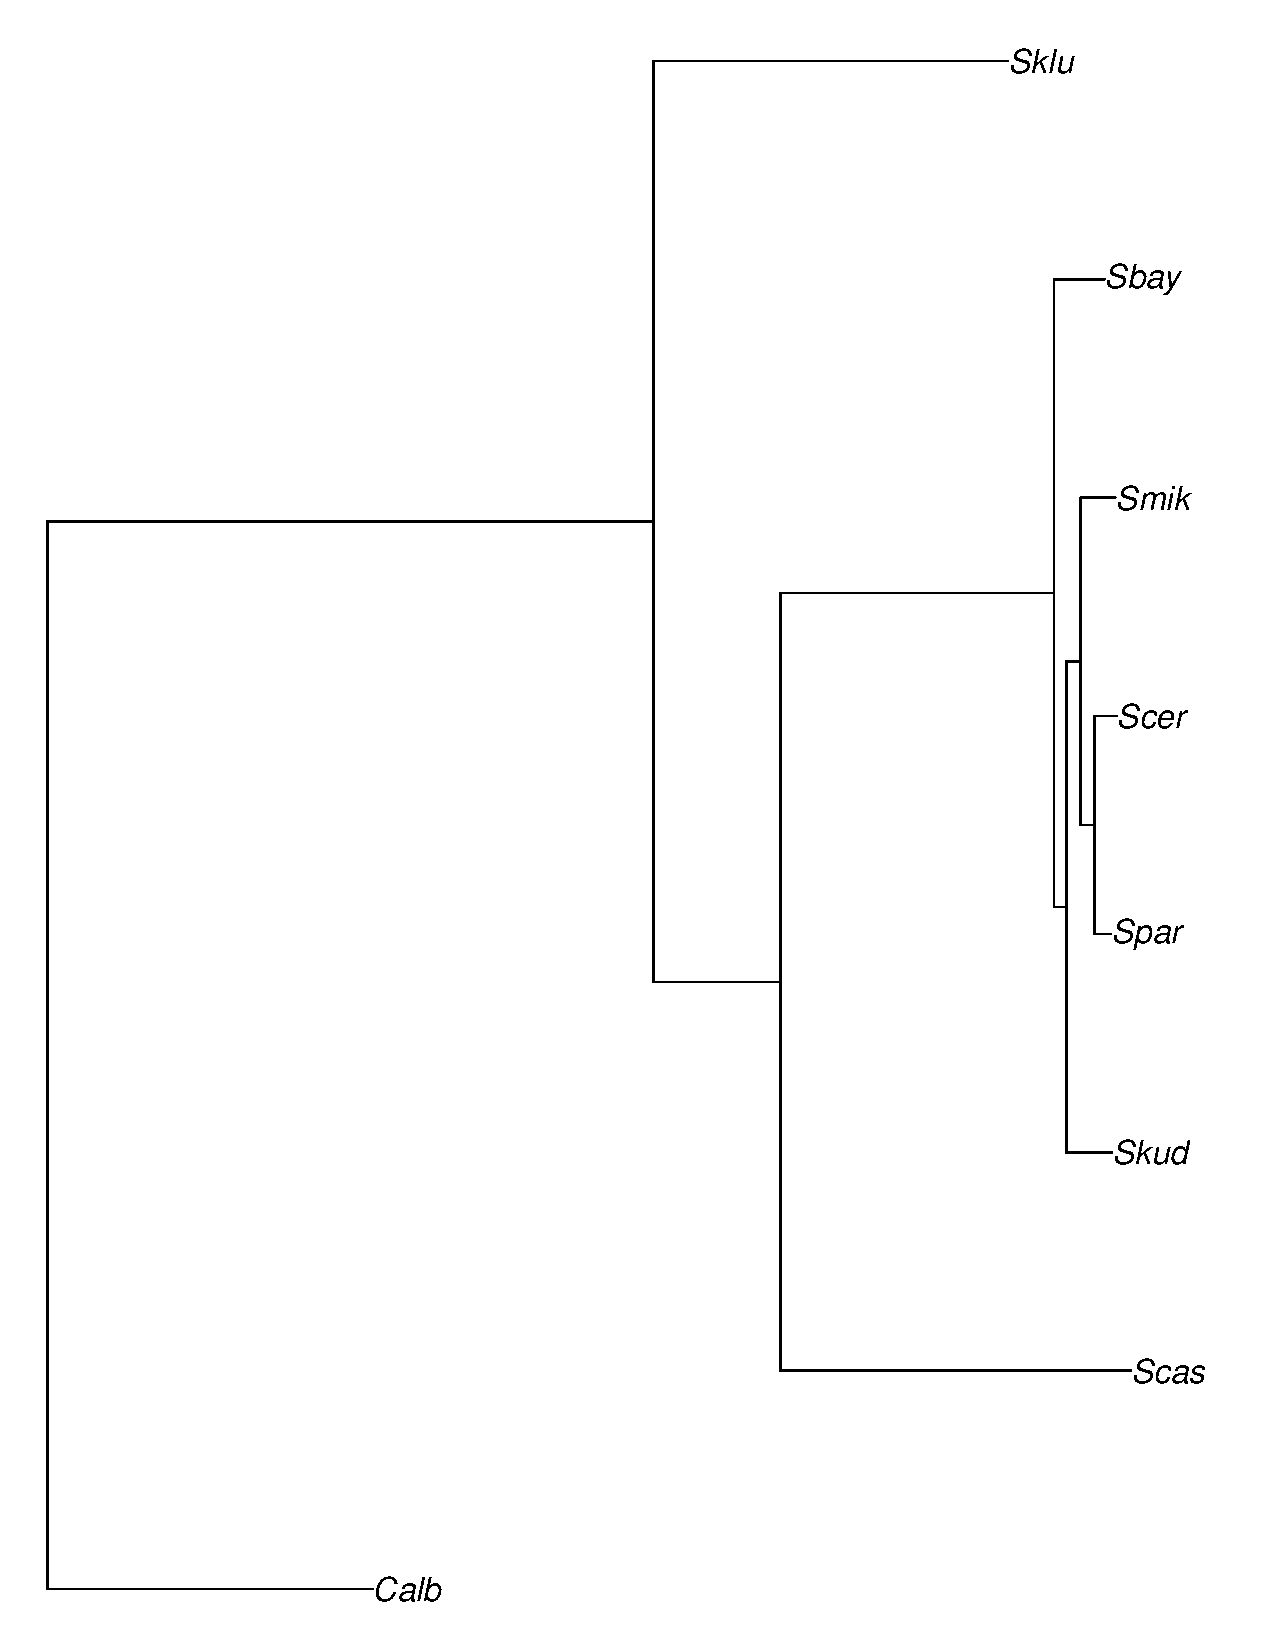
\includegraphics[width=0.8\textwidth,height=4cm]{besttree.pdf}
\end{figure}
%\begin{center}
%\line(1,0){250}
%\end{center}
%
%To check if the simulation is done correctly, here are some results. For simplicity, only 3 states (amino acids) are considered now. \\
%
%1. Check that the way to do simple simulation and to find the stationary probability is correct.\\
%
%Given the instantaneous substitution rate matrix $W$ for a Markov process with stationary probability vector $\mathbf{p}$ , $\mathbf{p}$ can be calculated by taking any row of the matrix $\exp(Wt)$ where $t$ is big enough to guarantee that the process has already reached stationarity. \\
%
%On the other hand, if $W$ comes from the mutation and fixation processes, then $\mathbf{p}$ can also be found by S-H's formula of stationary probabilities
%\begin{equation}
%\frac{p_i}{p_j} = (\frac{f_i}{f_j})^{\nu} = \frac{W_{ji}}{W_{ij}}
%\label{eq:stationary}
%\end{equation}
%
%
%
%
%Comparing $\mathbf{p}$ calculated in both ways verifies that S-H's formula is accurate. Next we compare $\mathbf{p}$ calculated from the simulation with that from either of the formulae. The way I found $\mathbf{p}$ is as follows:\\
%\begin{enumerate}
%\item Do simulations with long enough time so that there are at least $10,000$ substitutions in the simulated chain.
%\item Cut off the first 100 observations, before the time when the process reaches stationarity.
%\item Find the average time $\bar{t}$ taken for a certain number of substitutions (for example, 10), and record the state of the chain when the amount $\bar{t}$ of time passed.
%\item Find the frequency of the observed states, hence the approximation of $\mathbf{p}$.
%\end{enumerate}
%
%\begin{center}
%\line(1,0){250}
%\end{center}
%
%Following are some results.\\
%\begin{enumerate}
%\item Let $W$ be the substitution rate matrix between all the protein with 2 sites. Since there are only 3 states for each site, total number of protein is 9. Hence the dimension of the matrix $W$ is $9\times 9$.\\
%\begin{figure}[here]
%\centering
%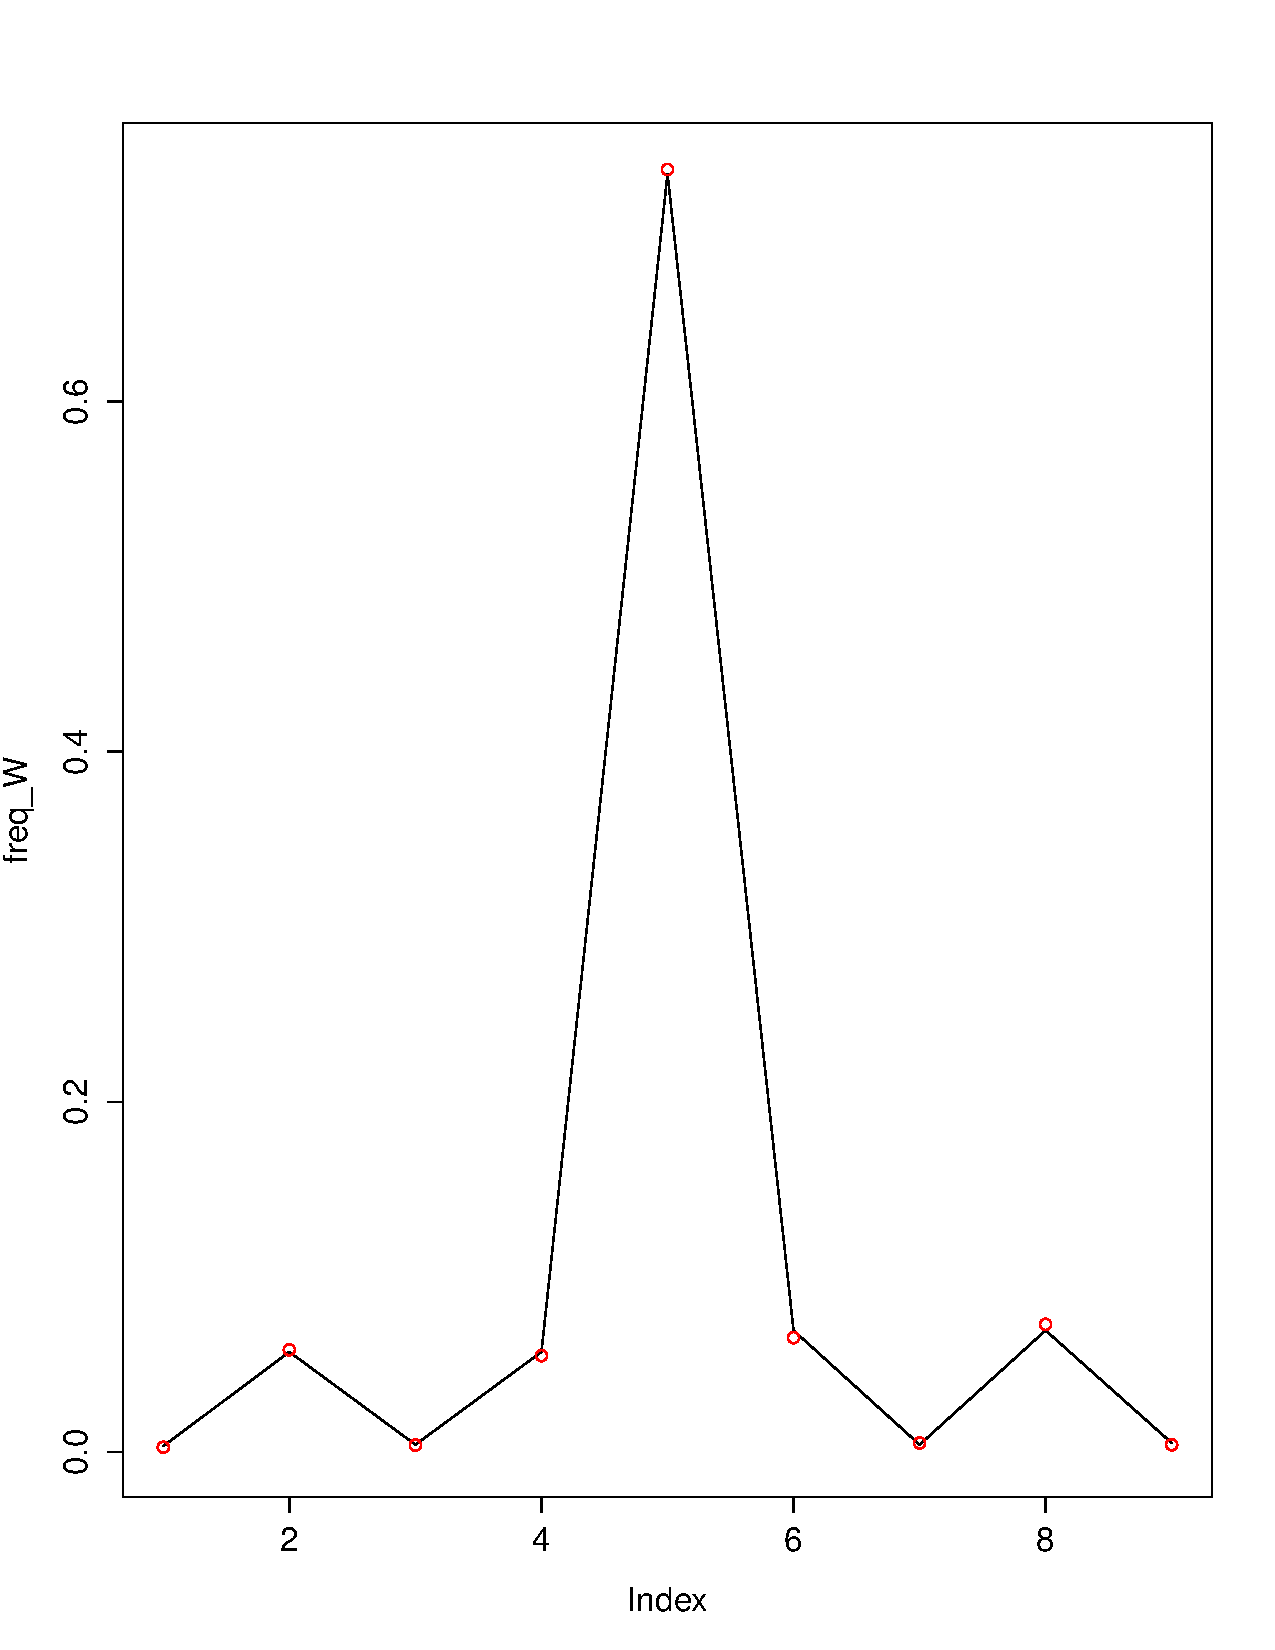
\includegraphics[scale=0.2]{freq_simple_sim.pdf}
%\caption{Stationary probabilities with 2 sites}
%\label{fig:freq2sites}
%\end{figure}
%
%In Figure~\ref{fig:freq2sites} on page ~\pageref{fig:freq2sites} the solid line connects the values of stationary probabilities for each state from theoretical calculation, and the red circles from simulation. \\
%%Obviously the simulation is done correctly and analyzed correctly in this case.\\
%
%\item Another simulation is done with 2 sites (3 states for each site) for each protein, starting with $(1,2)$, with optimal protein $(2,2)$, selection coefficient  0.1, running time $10^9$, sites dependent. The stationary probabilities are:
%\begin{table}[here]
%\begin{center}
%\begin{tabular}{rrrrrrrrrr}
%  \hline
%  1 & 2 & 3 & 4 & 5 & 6 & 7 & 8 & 9 \\ 
%  \hline
% 0.003364677 & 0.057514946 & 0.004235888 & 0.058025656 & 0.727881756 & 0.069636795 & 0.004130742 & 0.070132484 & 0.005077057 \\ 
%0.003324449 & 0.057134781 & 0.004132447 & 0.057134781 & 0.730153540 & 0.069429813 & 0.004132447 & 0.069429813 & 0.005127929 \\ 
%   \hline
%\end{tabular}
%\end{center}
%\end{table}
%
%First row is from simulation, second row is from Sella-Hirsh's formula. They are very close to each other. The number of steps in this simulation is $669061$, which is relatively big.\\
%
%\item A simulation with 3 sites and 3 states for each site confirmed the correctness of simulation. The chain starts with $(1,1,1)$, with optimal protein $(2,2,2)$, selection coefficient $0.01$, running time $10^8$, sites dependent. The number of observations is $216126$. Figure~\ref{fig:freq3sites} on page ~\pageref{fig:freq3sites} is a plot of stationary probabilities from both simulations and Sella-Hirsh's formula.
%\begin{figure}[here]
%\centering
%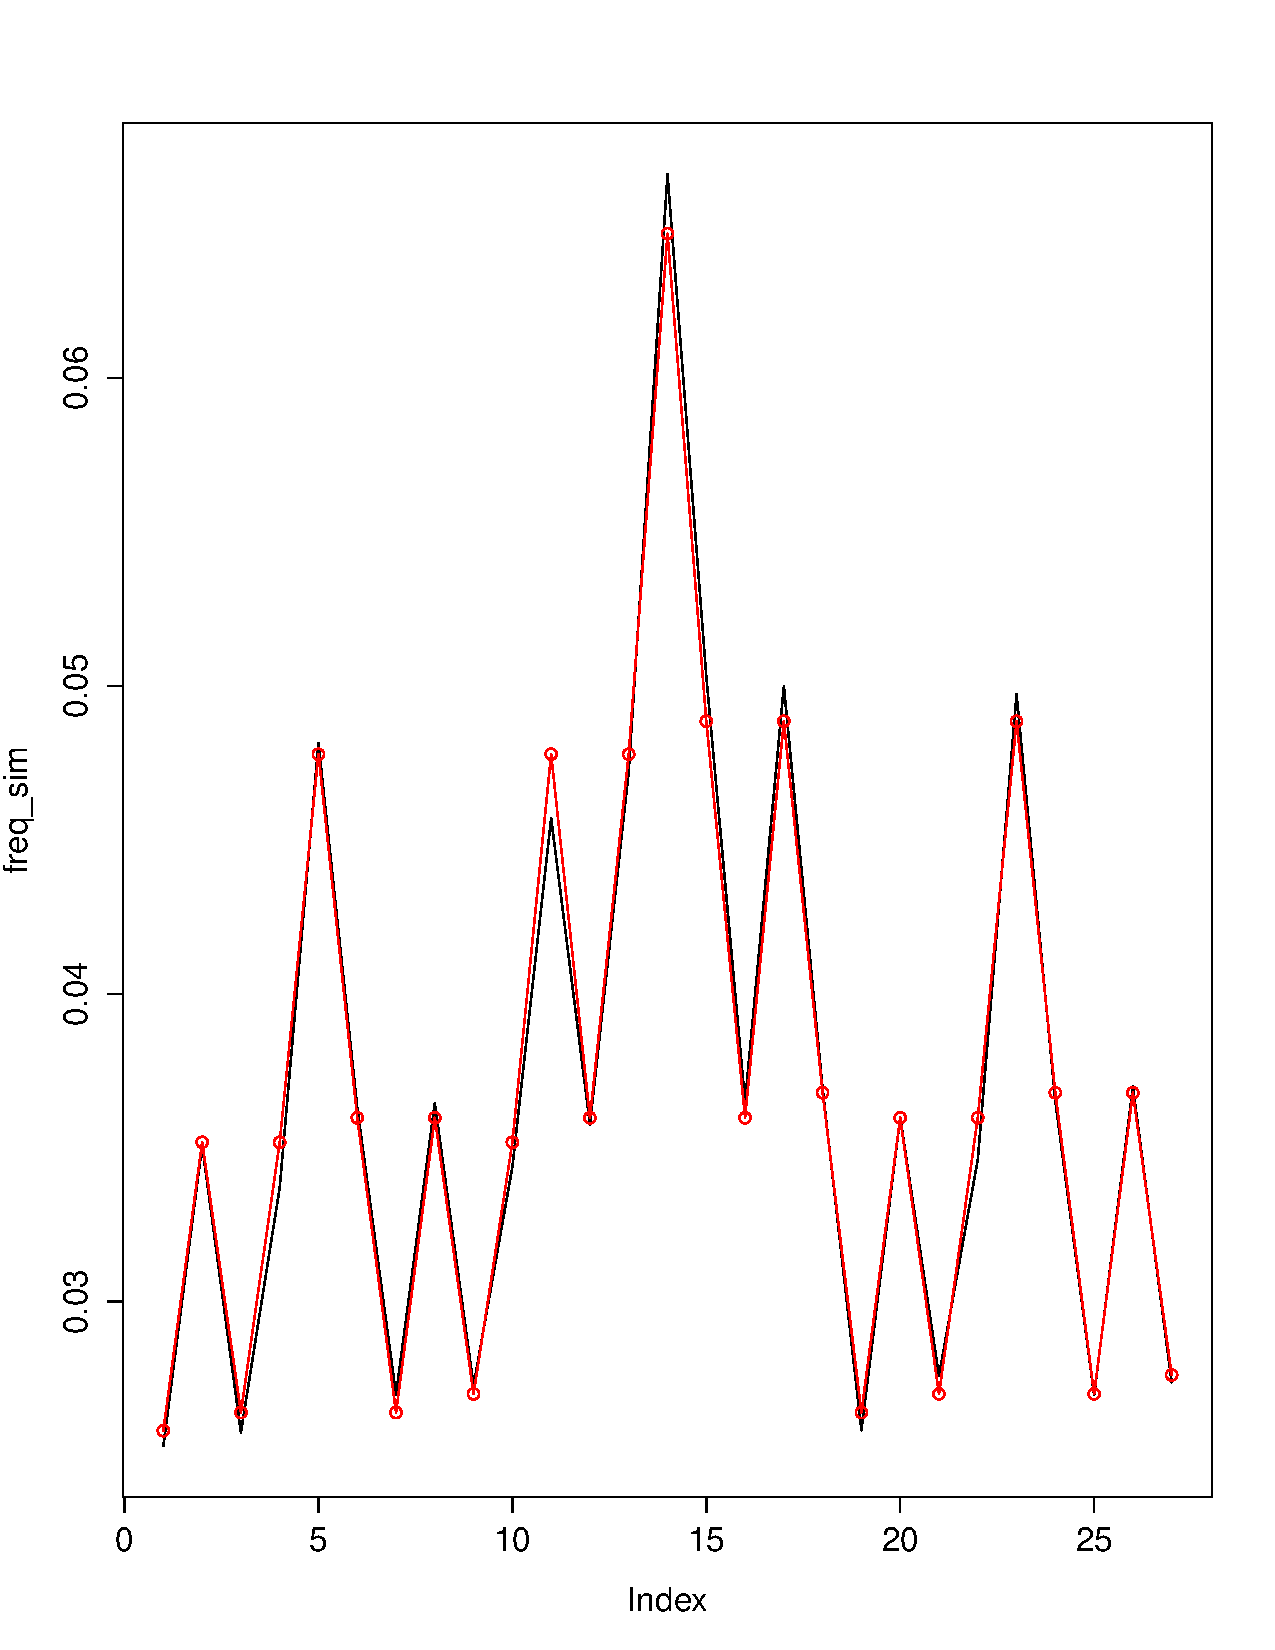
\includegraphics[scale=0.3]{3sites3states.pdf}
%\caption{stationary probabilities with 3 sites}
%\label{fig:freq3sites}
%\end{figure}
%
%\end{enumerate}
%
%\begin{center}
%\line(1,0){250}
%\end{center}
%
%Questions to answer next:
%\begin{enumerate}
%\item How to construct phylogeny from the simulated data?\\
%
%\item How to approximate the functionality (and other variables of concern) in the site-dependent case using site-independent case?\\
%
%In site-independent case, it's equivalent to assuming that every other site is at the optimal amino acid hence the functionality at those sites is 1. When the process has reached stationarity, if $\Phi$ is high and selection is strong, then the frequency of optimal amino acids will be high hence the assumption is reasonable. However, when $\Phi$ is small or selection is very weak, there tend to be more non-optimal amino acids at many sites.\\
%
%Consider the case when there are only 2 sites (amino acids) in the protein, fix the second site at a certain amino acid and let only site 1 change. How does site 2 affect the stationary distribution at site 1?\\
%
%From \eqref{eq:fitnessratio},
%\begin{equation}
%f_{ij} = \frac{f_i}{f_j} = \exp\Big(-\frac{A}{F_2}(e^{d_is_1} - e^{d_js_1})\Big)
%\label{eq:fitratioindep}
%\end{equation}
%In site-independent case, we assume site 2 is at the optimal amino acid, i.e. $F_2 = 1$, therefore
%\begin{equation}
%f_{ij}^{\text{ind}} = \exp\Big(-A(e^{d_is_1} - e^{d_js_1})\Big)
%\end{equation}
%
%The relationship between the two fitness ratios is
%\begin{equation}
%f_{ij}^{\text{ind}} = (f_{ij})^{F_2}
%\end{equation}
%
%If site 2 is not at the optimal amino acid, then $F_2 < 1$. Now consider the fitness ratios between an amino acid ($aa_i$) and the optimal amino acid ($aa_o$).\\
%\begin{eqnarray}
%f_{io} & = & \exp\Big(-\frac{A}{F_2}(e^{d_is_1} - 1)\Big)\\
%f_{io}^{\text{ind}} & = & (f_{io})^{F_2}
%\end{eqnarray}
%Since $f_{io} < 1$, $f_{io}^{\text{ind}} > f_{io}$, the fixation probability from an arbitraty amino acid to the optimal amino acid is higher in the site-dependent case. In other words, the selection strength at one site is {\bf higher} when other sites are not at the optimal amino acids.\\
%
%Let's see what happens with stationary distributions under site-independent and -dependent cases. From \eqref{eq:stationary}, 
%\begin{equation}
%\frac{p_i}{p_o} = \big(\frac{f_i}{f_o}\big)^\nu = (f_{io})^\nu
%\end{equation}
%Therefore 
%\begin{equation}
%(\frac{p_i}{p_o})^{\text{ind}} = (f_{io}^{\text{ind}})^\nu = (\frac{p_i}{p_o})^{F_2} > \frac{p_i}{p_o}
%\end{equation}
%
%This result could easily be generalized when the functionality $F_S$ is known for othere sites and only one site is changing, with $F_2$ replaced by $F_S$. Simulations also verified the relation.\\
%
%Rewriting the equation \eqref{eq:fitnessratio}, we can see
%\begin{equation}
%\frac{f_i}{f_j} = \exp\Big[-A\Big(e^{d_k^i s_k - \ln F_S} - e^{d_k^j s_k -  \ln F_S}\Big)\Big]
%\end{equation}
%What does this reflect the effect of $F_S$ on selection strength at site $k$?\\
%
%The most essential and what we are most interested in are the fixation rates from one protein to another, under both site-dependent and site-independent cases. If this is clear, the substitution rates and stationary distribution will follow, also the mean fitnesses. On the other hand, fixation probability is a function of fitness ratio, which also determines the stationary probabilities.\\
%
%Now we already know how to express the fitness ratio in site-dependent case in terms of that in site-independent case, with functionality at other sites as exponent, when there is only one site that is different between two proteins. \\
%
%To get the fitness ratio between any two proteins, we could use proteins that are one site away from them as bridges and represent the ratio as a product of several ratios we already know. For example:
%
%\begin{eqnarray*}
%\frac{f_{AA}}{f_{BB}} & = & \frac{f_{AA}}{f_{AB}} \cdot \frac{f_{AB}}{f_{BB}}\\
%\frac{f_{AA}}{f_{AB}} & = &(\frac{f^2_A}{f^2_B})^{-F_A}\\
%\frac{f_{AB}}{f_{BB}} & = &(\frac{f^1_A}{f^1_B})^{-F_B}
%\end{eqnarray*}
%
%If furthermore, the selection coefficients at the first and second positions are the same, then $\frac{f^2_A}{f^2_B} = \frac{f^1_A}{f^1_B} = \frac{f_A}{f_B}$ in site-independent case. Therefore
%\begin{equation*}
%\frac{f_{AA}}{f_{BB}} = (\frac{f_A}{f_B})^{-F_A-F_B}
%\end{equation*}
%
%If there are more than 2 sites that are different, then there need to be more than one intermediate proteins to relate them together. For example,
%\begin{equation*}
%\frac{f_{AAA}}{f_{BBB}} = \Big(\frac{f_A}{f_B}\Big)^{-F_{AA}-F_{AB}-F_{BB}}
%\end{equation*}
%However, if the selection coefficients are not the same across the sites, this relationship does not hold any more. The reason is that even fitness ratio in site-independent case depends on the selection coefficient at that particular site. 
%\end{enumerate}
%%Next step: set the mutation rate to be a different number, add mutation bias, move from amino acid level to codon level.
%
%\begin{center}
%\line(1,0){250}
%\end{center}
%
%Parameters to investigate during the optimization (optimx):\\
%\begin{enumerate}
%\item $s, \Phi, C, q, N_e$, some of them are correlated to each other and cannot be split separately
%\item tree topologies (at different extremes), branch lengths, number of tips
%\item ancestral sequences --- stationary, uniform, same sequence as used in the simulation
%\end{enumerate}
%
%Hessian matrix, variance, information; confidence interval, bootstrapping; ...
%
%\begin{center}
%\line(1,0){250}
%\end{center}
%
%Meeting on Thursday, Mar 8, 1012.
%\begin{enumerate}
%\item Do the plots of MLE bias with respect to number of sites (200, 400, 800 or more in between) : first, fix other parameters, estimate $s$; second, estimate $\Phi$ while fix other parameters. Do this for trees with 4 tips and 8 tips.
%\item Estimate the composite parameter.
%\item Instead of giving the equilibrium frequencies, make it depend on the parameters as from Sella-Hirsh's formula, and do the optimization that way.
%\item Let $s$ vary according to Gamma distribution instead of being fixed, and estimate the Gamma parameter(s).
%\end{enumerate}
%
%Profiling R code:
%
%> Rprof(file="rprof.out")
%> R command
%> Rprof(NULL)
%
%under unix, use command:
%R CMD Rprof rprof.out
\end{document}
